\documentclass[12pt,a4paper]{article}
\usepackage[latin1]{inputenc}
\usepackage[english]{babel}
\usepackage{amsmath}
\usepackage{amsfonts}
\usepackage{amssymb}
\usepackage{multicol}
\usepackage{listings}
\usepackage{xcolor}
\usepackage{parskip}
\usepackage{graphicx}
\author{Stijn Rosaer}
\title{Microservices - manual}
\date{November 27 2018}
\begin{document}
\maketitle
\section{Requirements}
This project is based on the python 3.6 standard. Please make sure that the correct version is available before installing the nessesary packages and running the program.\\

All required packages and dependencies will be installed when compiling the docker images. To install en start the service run following command from the app folder: docker-compose -f docker-compose-dev.yml up -d --build. This will install all necessary images with the correct version of dependencies.\\

To create a full working website with everything online, please run start.sh in the app folder. It is important that docker is able to run without sudo rights.

When browsing to http://localhost you will reach the home page of the website.\\

\pagebreak
There are multiple possibilities that allow to initialize databases, and seed them with data.\\
The API from delijn is used to fill the stops with their city and names. The lines on which they are is requested every time a detailed overview of a top is requested.\\

docker-compose -f docker-compose-dev.yml (followed by)
\begin{itemize}
\item run users python manage.py recreate-db
\item run users python manage.py seed-db
\item run scores python manage.py recreate-db
\item run scores python manage.py load-stops
\item run scores python manage.py seed-stops
\item run scores python manage.py seed-vehicles
\end{itemize}

This will reate all databases and fill them with dummy data.

\section{Containers}
\subsection{client}
The client containers runs the react server that is responsible for the user interface that is used to display the website. The app.py contains every route that is possible and the home page. In the components' folder I placed all the other pages and elements that are used on that pages. Taking into account that some elements can be shared on multiple pages.\\

To make the request to the back-end, I used axios since this is easy to set up in react and allows easy response handling.\\
To create a good-looking website, I used bulma. This allows a quick creation of styled elements.

\subsection{scores}
The scores' container contains everything to make the service functional. In here, I placed all the functions that handle the requests to preform various operations. Using this container, it is possible to get an average score, add busses or trams, rate something or remove a vehicle that you added and no one else has rated.\\

You have to be logged-in to remove/add a vehicle or rate something.

\subsection{scores-db}
The scores-db container contains the postgresql database that holds all ratings and entities that can be rated.\\

\begin{multicols}{2}
\underline{stops}\\
\begin{tabular}{c|c}
\textbf{Column} & \textbf{Type}\\
id & intiger\\\hline
name & string\\\hline
entity & string\\\hline
city & string
\end{tabular}


\underline{stopscores}\\
\begin{tabular}{c|c}
\textbf{Column} & \textbf{Type}\\
id & intiger\\\hline
score & intiger\\\hline
username & string
\end{tabular}

\underline{vehicles}\\
\begin{tabular}{c|c}
\textbf{Column} & \textbf{Type}\\
id & intiger\\\hline
type & string\\\hline
username & string
\end{tabular}

\underline{vehiclescores}\\
\begin{tabular}{c|c}
\textbf{Column} & \textbf{Type}\\
id & intiger\\\hline
score & intiger\\\hline
username & string
\end{tabular}
\end{multicols}

\subsection{users}
The users container handles all user and authentication request. This includes the registration, login and logout.

\pagebreak
\subsection{users-db}
The users-db container contains the postgresql database that holds all user data.\\

\begin{center}
\underline{users}\\
\begin{tabular}{c|c}
\textbf{Column} & \textbf{Type}\\
id & intiger autoincrement\\\hline
username & string\\\hline
email & string\\\hline
password & string (hashed)\\\hline
logedin & boolean
\end{tabular}
\end{center}

\subsection{nginx}
To make sure that all traffic is correctly routed and the user doesn't need to enter a port number in the url, I chose to use nginx in an extra container. This allows to define where each request should be forwarded to.

\pagebreak
\section{API calls}
\subsection{Users}
Url: $/users$\\
Method: GET\\
Parameters: /\\
Response: json formatted users\\

Url: $/auth/register$\\
Method: GET\\
Parameters: 
\begin{itemize}
\item username
\item email
\item password
\end{itemize}
Response: success object\\
Info: user will be added to the users table\\

Url: $/auth/login$\\
Method: POST\\
Parameters: 
\begin{itemize}
\item username
\item password
\end{itemize}
Response: success object\\
Info: verification if username and password combination is correct\\

Url: $/auth/logout$\\
Method: POST\\
Parameters: \begin{itemize}
\item username
\end{itemize}
Response: success object\\
Info: set logout to true\\

\subsection{Scores}
Url: $/scores/search/s/id/<id>$\\
Method: GET\\
Parameters: stop id\\
Response: json list of stops with requested id\\

Url: $/scores/search/s/line/<line>/<entity>$\\
Method: GET\\
Parameters:\begin{itemize}
\item line number
\item province
\end{itemize}
Response: json list of stops on requested line and entity\\

Url: $/scores/search/s/city/<city>$\\
Method: GET\\
Parameters:\begin{itemize}
\item city
\end{itemize}
Response: json list of stops in requested city\\

Url: $/scores/search/v/id/<id>$\\
Method: GET\\
Parameters:\begin{itemize}
\item vehicle id
\end{itemize}
Response: json list of vehicles with requested id\\

Url: $/scores/search/v/type/<type>$\\
Method: GET\\
Parameters:\begin{itemize}
\item vehicle type
\end{itemize}
Response: json list of vehicles of requested type\\

\pagebreak
Url: $/scores/vehicle/remove$\\
Method: POST\\
Parameters:\begin{itemize}
\item vid (vehicle id)
\end{itemize}
Response: success object if vehicle is correctly removed\\

Url: $/scores/vehicle$\\
Method: POST\\
Parameters:\begin{itemize}
\item vid (vehicle id)
\item score
\item username
\end{itemize}
Response: success object with vehicle id if score is set\\

Url: $/scores/stop$\\
Method: POST\\
Parameters:\begin{itemize}
\item sid (stop id)
\item score
\item username
\end{itemize}
Response: success object with stop id if score is set\\

Url: $/scores/stops/avg$\\
Method: GET\\
Parameters: /\\
Response: success object with list of top and worst stops and their average score\\

Url: $/scores/vehicles/avg$\\
Method: GET\\
Parameters: /\\
Response: success object with list of top and worst vehicles and their average score\\

Url: $/scores/vehicles/id/<id>$\\
Method: GET\\
Parameters: \begin{itemize}
\item vehicle id
\end{itemize}
Response: json object with all vehicle details of requested id including list of all ratings\\

Url: $/scores/stops/id/<id>$\\
Method: GET\\
Parameters: \begin{itemize}
\item vehicle id
\end{itemize}
Response: json object with all stop details of requested id including list of all ratings\\

Url: $/scores/addvehicle$\\
Method: POST\\
Parameters: \begin{itemize}
\item id (vehicle id)
\item type
\item username
\end{itemize}
Response: success object if vehicle is correctly created and added to the database\\



\pagebreak
\section{Design choices}
I make several choices when designing this system. For the back-end, I decided to devide the service in more logical containers then requested. I splitted the databases to make a clear separation between the functionality. This is also important for scalability and security. If the security of the scores' database would be compromised, they wouldn't have access to the user data. The passwords are also not stored in plain text but hashed using a build in function.\\

The API's are splitted in the same way as the databases to keep an overview of what functionality can be found where. This way, it would also be possible to use the users' container for another application or even use it for multiple applications at the same time.\\

I decided to make use of nginx as service to route the traffic to the correct microservice. This makes it possible to define what request should end where. This prevents that the user of my service has to enter the port numbers for every request in the url.\\

Because everything is contained in docker, there are no issues with dependencies or versions of plugins. Everything is defined in the docker files and the requirements for every service. The docker-compose-dev.yml is a place where all the settings for every microservice is defined such as what port the services should be accessed on, what directory they can be found in, what docker file to use and the dependencies to other services.\\
This makes it really easy to install everything at once.

\pagebreak
\section{Website}
The website is made using react that is hosted in its own container and compiles the requested pages. To make the layout more attractive, I used bulma for styling and the build in components such as the stars for rating the stops and vehicles.\\
There are multiple pages that are explained below and images of them on the following pages. I provided multiple users that can be used.

\begin{itemize}
\item username: user1, password: 1111
\item username: user2, password: 2222
\end{itemize}


\subsection{Web pages}
\begin{itemize}
\item Home
\item[] Landing page with a short introduction
\item Stops
\item[] A page with two lists. One containing the top 50 rated stops and one containing the worst 50 stops
\item Vehicles
\item[] A page with two lists. One containing the top 50 rated vehicles and one containing the worst 50 vehicles. If logged in, this page will also show a button to add a vehicle
\item Add vehicle
\item[] A form that can be used to add a vehicle if logged in
\item Search
\item[] Several pages to search for stops and vehicles based on different parameters
\item Login / Logout / Register
\item[] These forms are used to log in, register of the button to logout
\pagebreak
\item Item specific information
\item [] This pages can be accessed by the info button on the lists. It will show all the possible information on a stop or vehicle including a list of all the rating of different people. If logged in, it is also possible to use the start to give a rating. When u are the creator of this vehicle and no one else has given a rating, u can remove the vehicle from the database.
\end{itemize}
\pagebreak

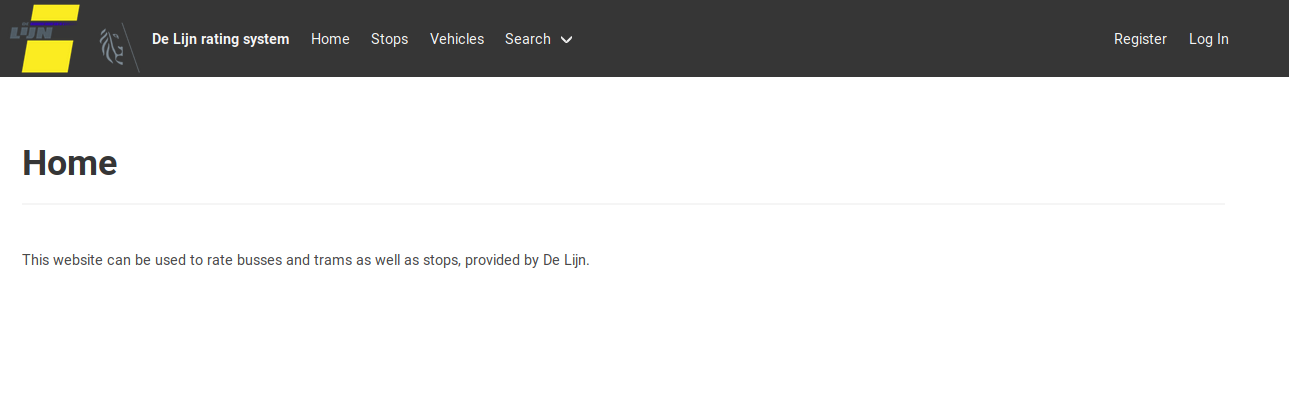
\includegraphics[scale=0.3]{home}\\
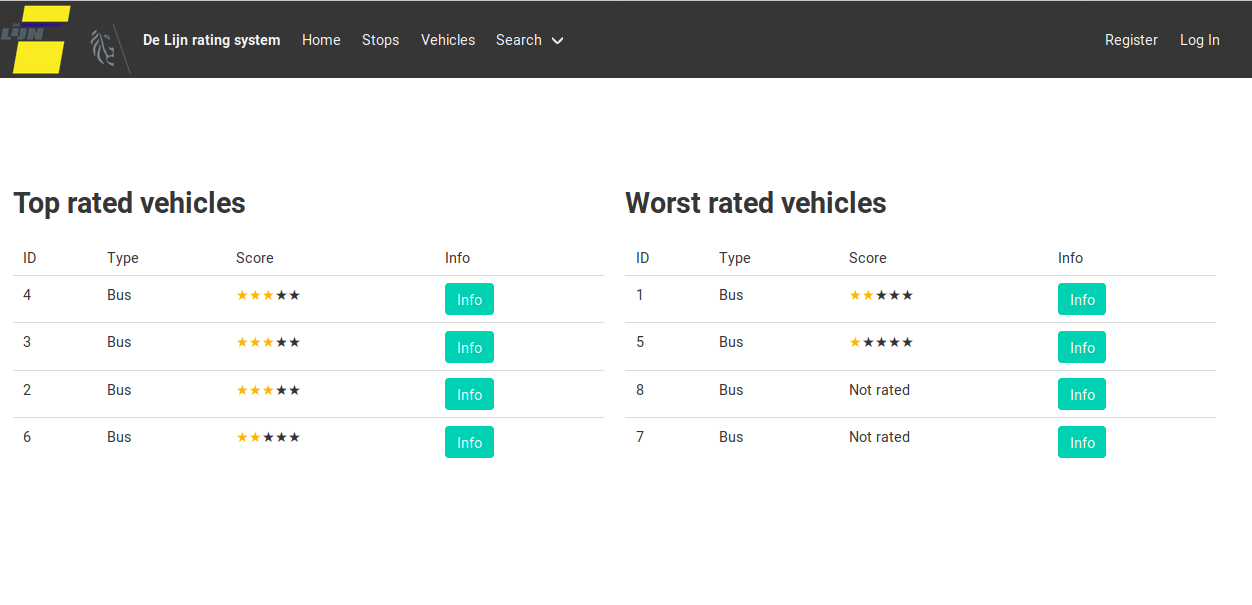
\includegraphics[scale=0.3]{vehicles}\\
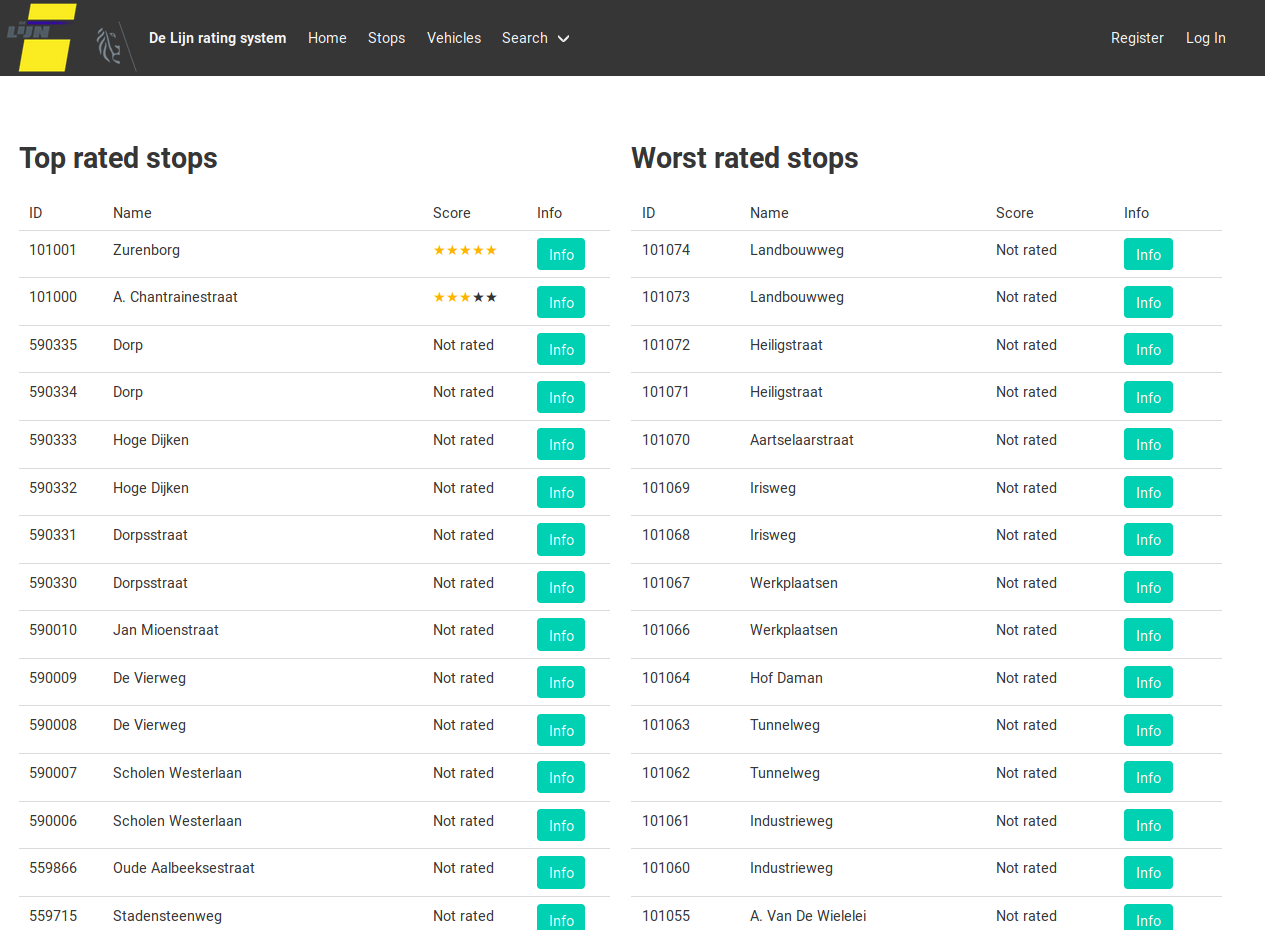
\includegraphics[scale=0.3]{stops}\\
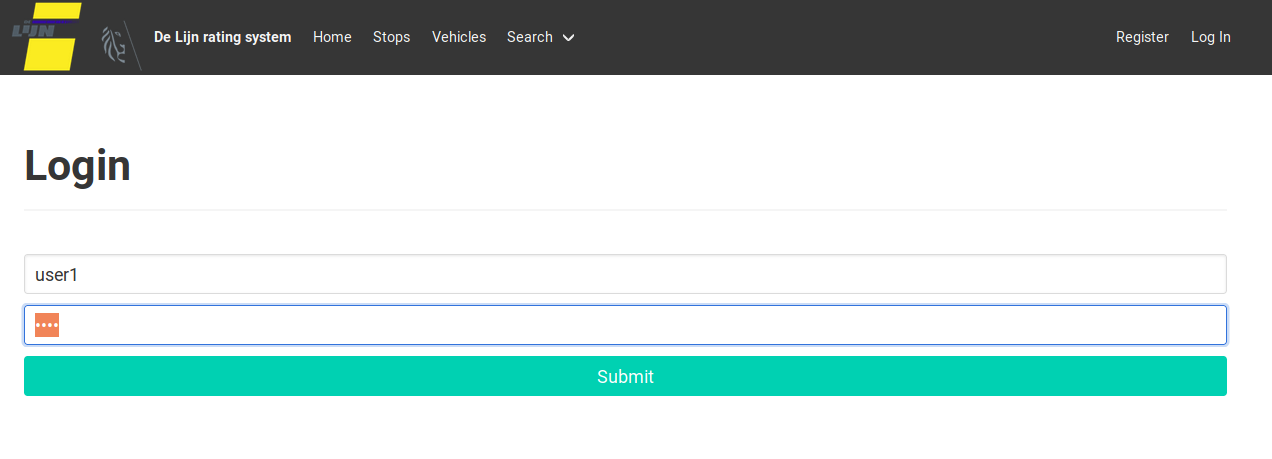
\includegraphics[scale=0.3]{login}\\
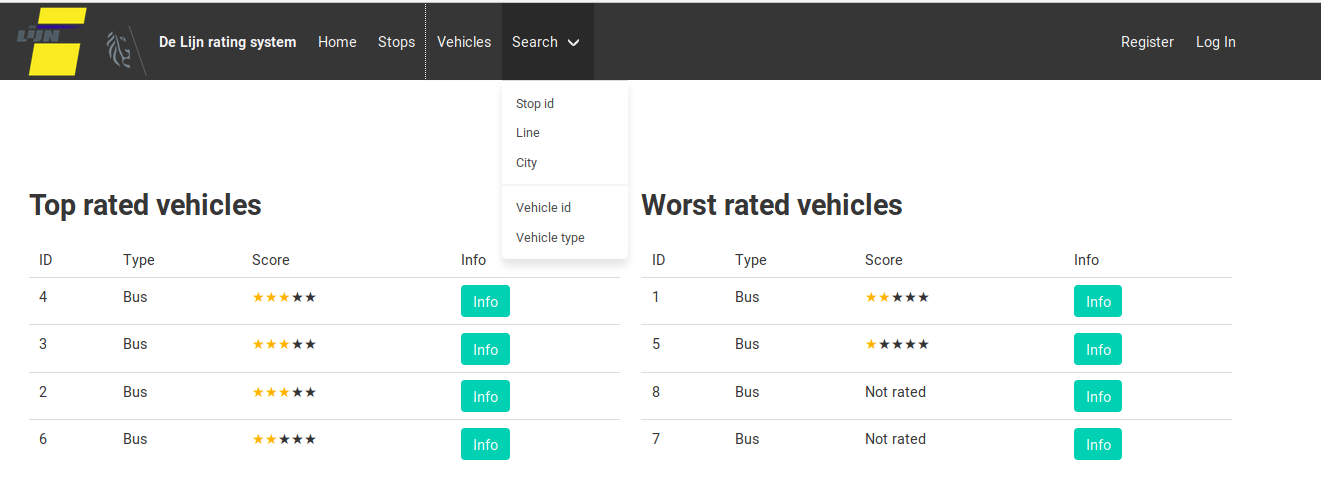
\includegraphics[scale=0.3]{search-bar}\\
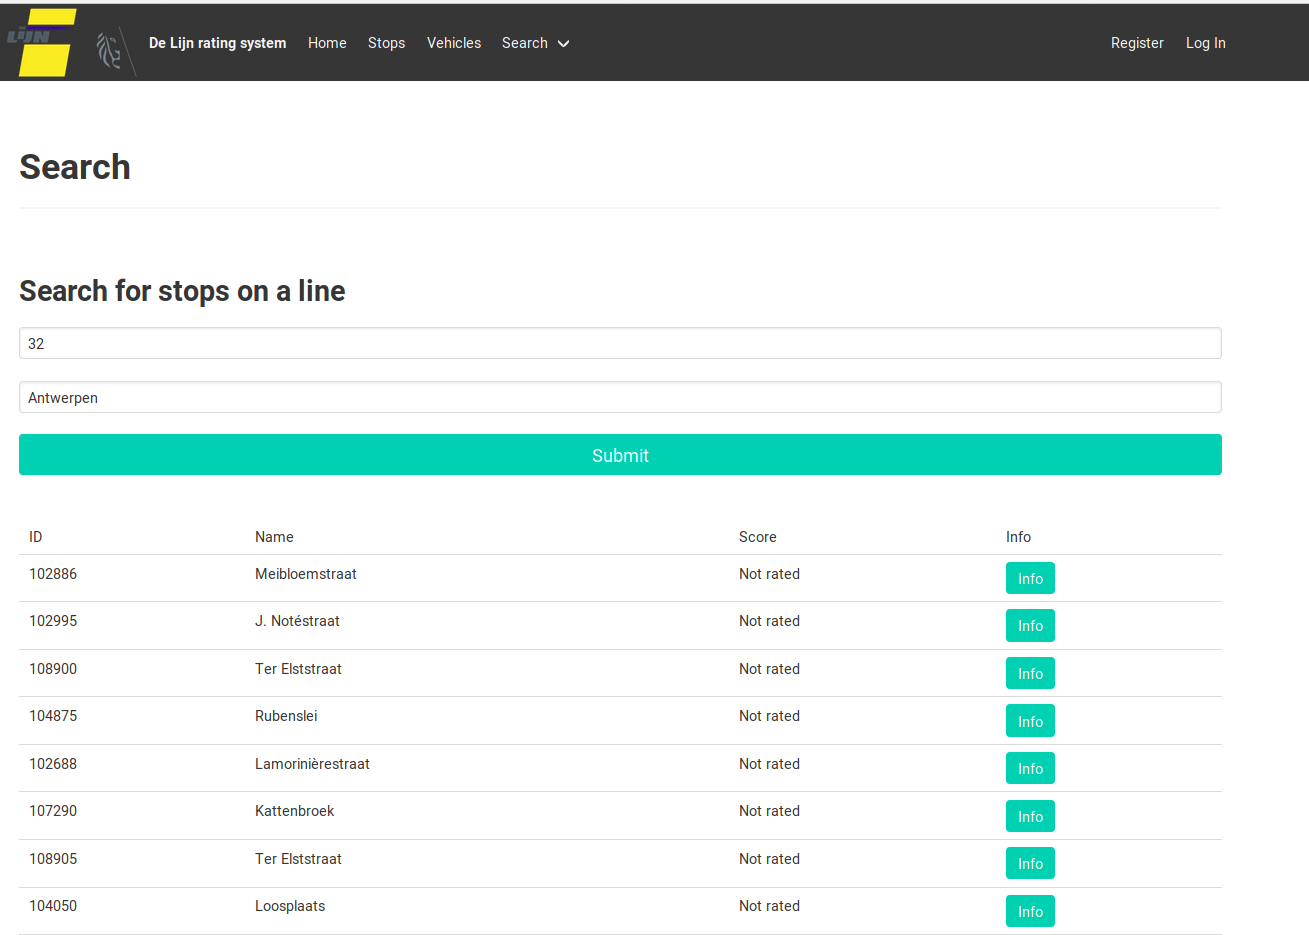
\includegraphics[scale=0.3]{search}\\
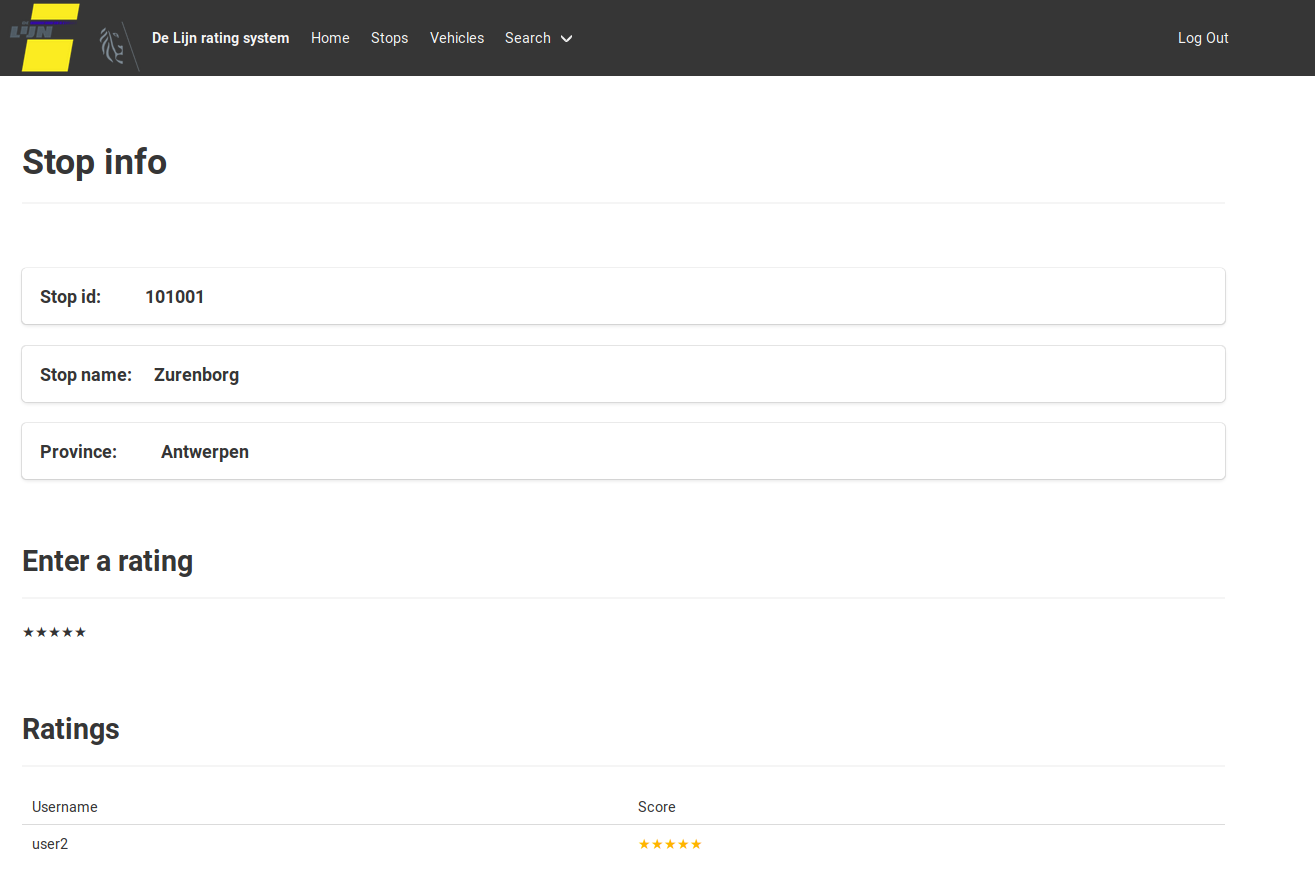
\includegraphics[scale=0.3]{stopInfo}\\
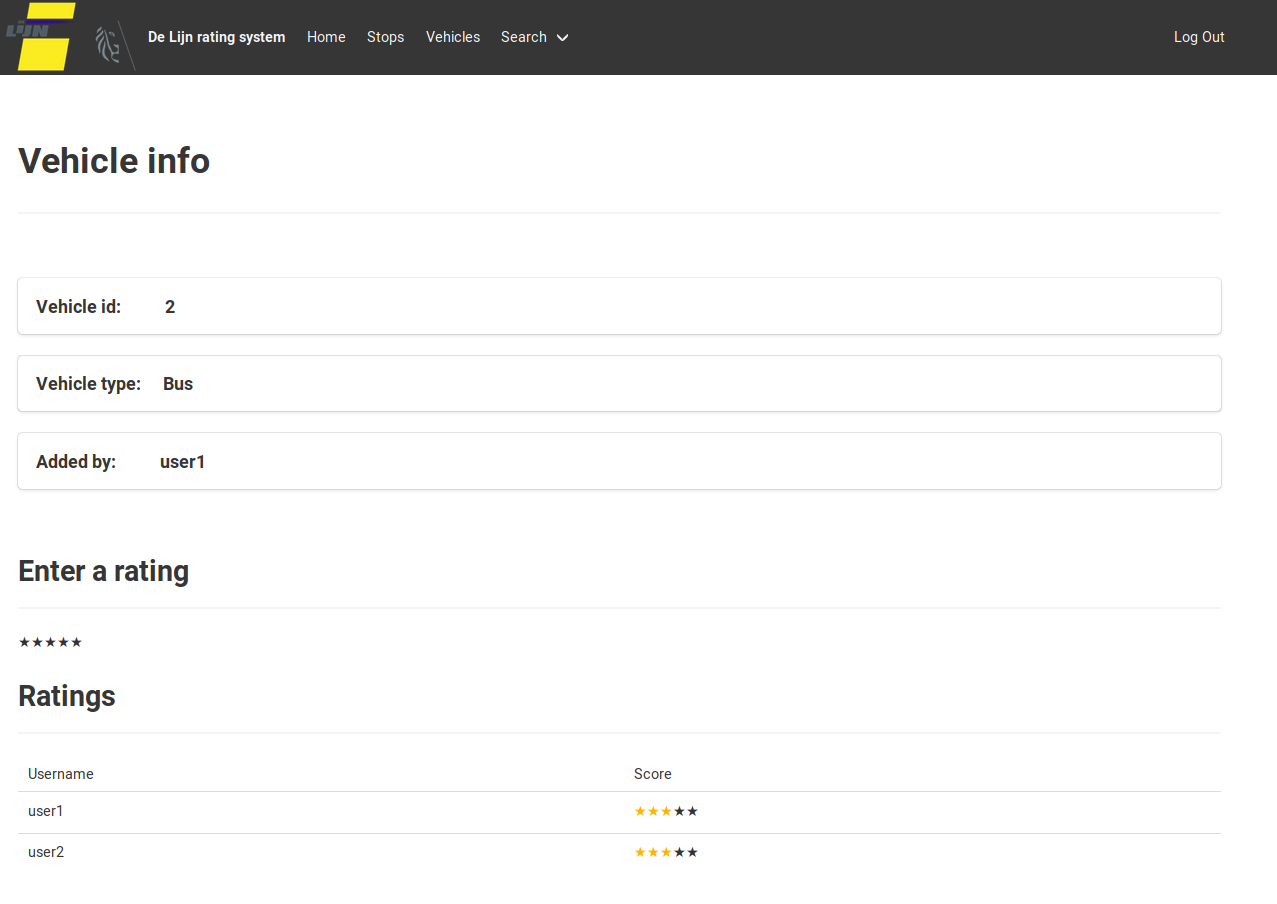
\includegraphics[scale=0.3]{vehicleInfo}\\
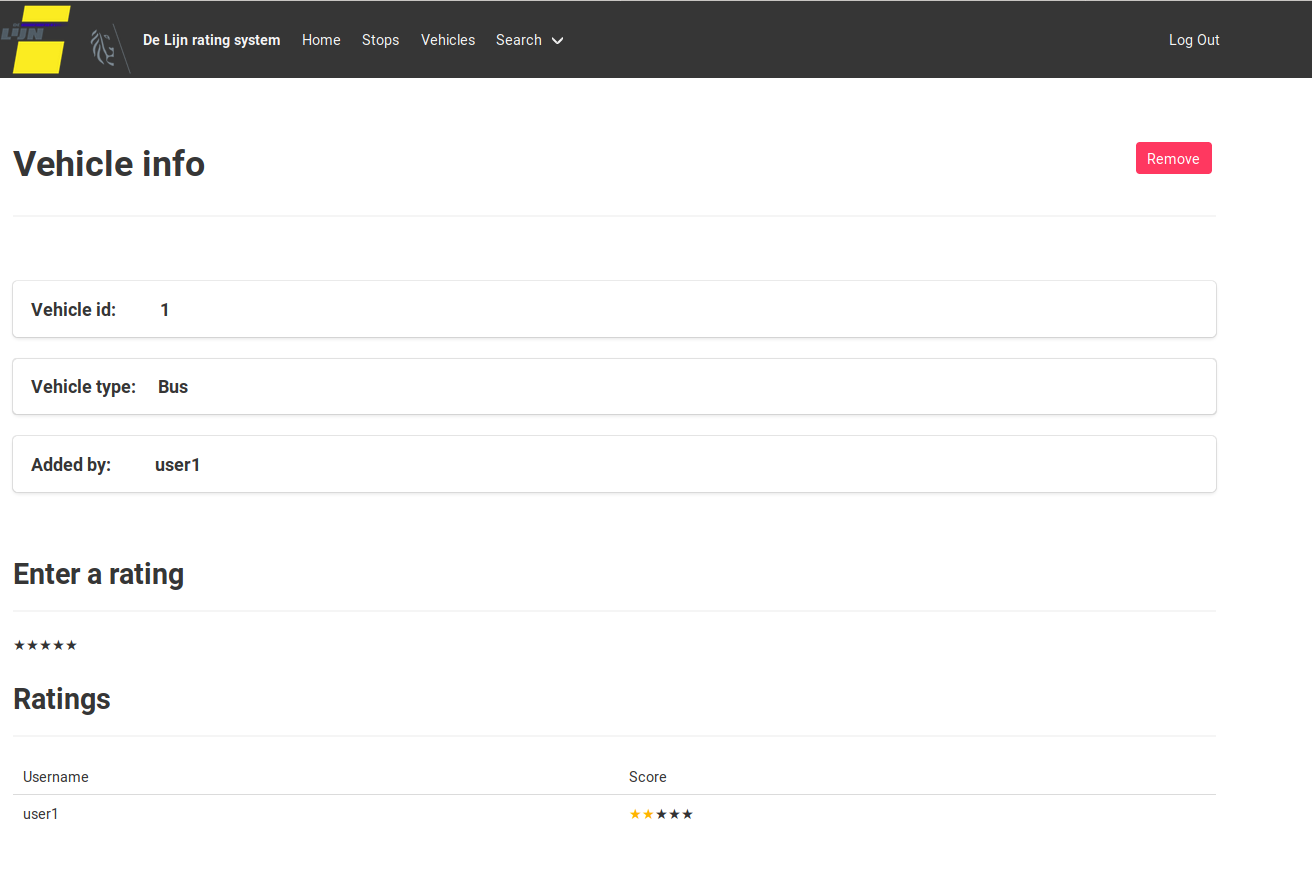
\includegraphics[scale=0.3]{vehicleRemove}
 


\end{document}